% Figure 1: fibre-preserving moves under a symmetry (inversion flip; linker exchange).
% Build (in this folder): pdflatex fig_moves  ->  fig_moves.pdf, included by ../paper/symmetry_fibres.tex
\documentclass[tikz,border=4pt]{standalone}
\usepackage{amsmath,amssymb}
\usepackage{lmodern}
\usepackage[T1]{fontenc}
\usetikzlibrary{arrows.meta,positioning}
\newcommand{\spec}{\operatorname{spec}}
\newcommand{\DS}{\mathrm{DS}}
\begin{document}
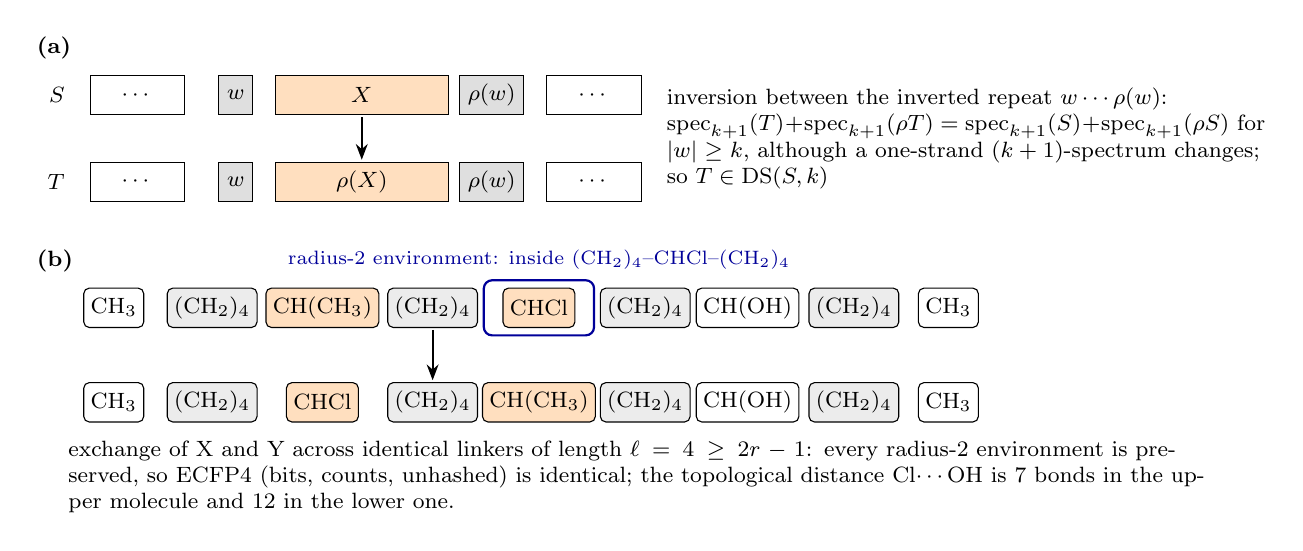
\begin{tikzpicture}[font=\small,
  seg/.style={draw, minimum height=0.5cm, inner sep=3pt, font=\footnotesize},
  rep/.style={seg, fill=gray!25},
  inv/.style={seg, fill=orange!25},
  atom/.style={draw, rounded corners=2pt, minimum height=0.5cm, inner sep=2.5pt, font=\footnotesize},
  lnk/.style={atom, fill=gray!15},
  lab/.style={font=\footnotesize, align=left, anchor=west}]
% ---------------- (a) inversion flip between an inverted repeat
\node[anchor=west, font=\bfseries\footnotesize] at (-0.6,3.6) {(a)};
\node[anchor=east, font=\footnotesize] at (0.0,3.0) {$S$};
\node[seg, minimum width=1.2cm] (a1) at (0.8,3.0) {$\cdots$};
\node[rep] (w1) at (2.05,3.0) {$w$};
\node[inv, minimum width=2.2cm] (x1) at (3.65,3.0) {$X$};
\node[rep] (rw1) at (5.3,3.0) {$\rho(w)$};
\node[seg, minimum width=1.2cm] (a2) at (6.6,3.0) {$\cdots$};
\node[anchor=east, font=\footnotesize] at (0.0,1.9) {$T$};
\node[seg, minimum width=1.2cm] at (0.8,1.9) {$\cdots$};
\node[rep] at (2.05,1.9) {$w$};
\node[inv, minimum width=2.2cm] at (3.65,1.9) {$\rho(X)$};
\node[rep] at (5.3,1.9) {$\rho(w)$};
\node[seg, minimum width=1.2cm] at (6.6,1.9) {$\cdots$};
\draw[-{Stealth[length=2mm]}, thick] (3.65,2.72) -- (3.65,2.18);
\node[lab, text width=7.6cm] at (7.4,2.45) {inversion between the inverted repeat $w\cdots\rho(w)$:
  $\spec_{k+1}(T)+\spec_{k+1}(\rho T)=\spec_{k+1}(S)+\spec_{k+1}(\rho S)$ for $|w|\ge k$, although a
  one-strand $(k+1)$-spectrum changes; so $T\in\DS(S,k)$};
% ---------------- (b) exchange across repeated linkers
\node[anchor=west, font=\bfseries\footnotesize] at (-0.6,0.9) {(b)};
\foreach \y/\X/\Y in {0.3/CH(CH$_3$)/CHCl, -0.9/CHCl/CH(CH$_3$)} {
  \node[atom] at (0.5,\y) {CH$_3$};
  \node[lnk] at (1.75,\y) {(CH$_2$)$_4$};
  \node[atom, fill=orange!25] at (3.15,\y) {\X};
  \node[lnk] at (4.55,\y) {(CH$_2$)$_4$};
  \node[atom, fill=orange!25] at (5.9,\y) {\Y};
  \node[lnk] at (7.25,\y) {(CH$_2$)$_4$};
  \node[atom] at (8.55,\y) {CH(OH)};
  \node[lnk] at (9.9,\y) {(CH$_2$)$_4$};
  \node[atom] at (11.1,\y) {CH$_3$};
}
\draw[-{Stealth[length=2mm]}, thick] (4.55,0.02) -- (4.55,-0.62);
% a radius-2 ball around the CHCl carbon of the first molecule
\draw[blue!60!black, thick, rounded corners=3pt] (5.2,-0.05) rectangle (6.6,0.65);
\node[font=\scriptsize, blue!60!black, anchor=south] at (5.9,0.66) {radius-2 environment: inside (CH$_2$)$_4$--CHCl--(CH$_2$)$_4$};
\node[lab, text width=14.6cm] at (-0.2,-1.85) {exchange of X and Y across identical linkers of length
  $\ell=4\ge2r-1$: every radius-2 environment is preserved, so ECFP4 (bits, counts, unhashed) is identical;
  the topological distance Cl$\cdots$OH is $7$ bonds in the upper molecule and $12$ in the lower one.};
\end{tikzpicture}
\end{document}
